\documentclass[11pt]{article}
\usepackage[margin=1in]{geometry}
\usepackage[T1]{fontenc}
\usepackage{lmodern}
\usepackage{microtype}
\usepackage{amsmath,amssymb}
\usepackage{graphicx}
\usepackage{booktabs}
\usepackage[authoryear,round]{natbib}
\usepackage[font=small,labelfont=bf]{caption}
\usepackage{xcolor}
\usepackage{float}
\usepackage{placeins}
\usepackage{makecell}
\usepackage{array}
\setlength{\emergencystretch}{2em}
\usepackage[colorlinks=true,linkcolor=black,citecolor=black,urlcolor=black]{hyperref}

\setlength{\parskip}{3pt}
\renewcommand{\arraystretch}{1.12}
\newcommand{\Rtwo}{R^2}

\title{Predicting how long each choice takes\\[4pt]\large Decision time section, draft for the choice overload paper}
\author{Asif Rahman}
\date{4 November 2026}

\begin{document}
\maketitle

\begin{abstract}
\noindent Choice models are usually judged by the choices they predict. This section asks whether they can also say how long a particular choice will take. We used eight datasets that record both choices and decision times. The outcome is log time centered within each participant, so a prediction says which of a person's trials will take longer, not who is faster. In a confirmatory test, four features of the trial (the number of options, the best value, the gap to the runner up and the mean of the rest) predicted which trials took longer beyond the number of options alone in four of the eight datasets, and a law fitted to the other datasets carried over to three. In an exploratory comparison of 32 models, developed over three rounds and then scored on a sealed 30 percent of each dataset's participants, two look satisficing timed decisions as well as the four feature law. It is a search model whose one sensitivity is fitted to choices alone and which needs only a time slope to turn expected looks into time. The Bayes factors for no difference from the four feature law were 11 to 19 in three datasets, and its predictions were calibrated across the whole range of times. Races of accumulators with a fixed threshold predicted faster choices from larger trials and needed a threshold that rises with set size, and the likelihood of one race family had several optima that a first fit missed. On the vault, no model explained as much as 1 percent of the variance in the sums, and none clearly beat a constant time in the two tasks of our study or in three snacks, a flexible machine learning model included. Decision time follows the structure of the trial in a way a search model with an absolute standard can capture, but even the best models explain at most about a sixth of the variation between a person's trials.
\end{abstract}

\section{What this section asks}

A model of how people choose also implies how long they take. Times are recorded in most choice experiments but are rarely used to test choice models, which are fitted and compared on choices. This section asks two questions of every dataset in the paper that records times. The first is whether the structure of a trial, meaning how many options there are and how their values are spread, predicts which of a person's trials take longer. The second is whether a model of the choice process can predict each trial's time as well as that structure does, and which models can.

The first question was a confirmatory test, fixed in the analysis plan before any time was analysed in this way (Amendment 12). The second was exploratory. It allowed repeated rounds of model building on part of the data, followed by a single test on participants who had been held back from every round (Section~\ref{sec:models}).

\section{Data, outcome and score}
\label{sec:data}

\paragraph{Datasets.} Table~\ref{tab:data} lists the eight datasets. Two come from our own study, in which participants chose files and laptops from fixed displays of 8 to 32 options scored by a rubric. Three are open datasets of choices from trials with many options. In the first, snacks are chosen from sets of 9 to 36 items \citep{thomas2021}. In the second, snacks are chosen from 4, 9 or 16 items within three seconds \citep{reutskaja2011}. In the third, sums of money have to be worked out from arithmetic and are chosen from 10 to 40 options \citep{caplin2011}. The last three are open eye tracking datasets of choices between two or three foods \citep{krajbich2010,krajbich2011,folke2016}, in the versions prepared by \citet{thomas2019}. Values were rescaled to run from 0 to 1 using the ends of each dataset's value scale. Trial inclusion follows the amendment that first used each dataset.

\begin{table}[t]
\centering
\footnotesize
\setlength{\tabcolsep}{4pt}
\caption{Datasets with decision times. The labels are used throughout the paper.}
\label{tab:data}
\begin{tabular}{llcll}
\toprule
Dataset & Source & Set sizes & Time recorded & Values \\
\midrule
Our study, files & This study & 8, 16, 32 & time on the trial page & rubric scores \\
Our study, laptops & This study & 8, 16, 30, 32 & time on the trial page & rubric scores \\
Snacks at a glance & \citet{thomas2021} & 9, 16, 25, 36 & response time & ratings \\
Snacks in three seconds & \citet{reutskaja2011} & 4, 9, 16 & response time, 3 s limit & ratings \\
Sums worked out & \citet{caplin2011} & 10, 20, 40 & final selection & sums to work out \\
Two foods & \citet{krajbich2010} & 2 & response time & ratings, 0 to 10 \\
Three foods & \citet{krajbich2011} & 3 & response time & ratings, 0 to 10 \\
Three snacks & \citet{folke2016} & 3 & response time & ratings, 0 to 10 \\
\bottomrule
\end{tabular}
\end{table}

\paragraph{Outcome.} The outcome is log decision time in seconds, centered within participant,
\begin{equation}
y_{it} = \log t_{it} - \frac{1}{T_i}\sum_{s} \log t_{is},
\end{equation}
where the sum runs over the $T_i$ included trials of person $i$. Centering removes how fast each person is, so a model is judged on which of a person's trials take longer and not on who is faster. Every model's predictions are centered within person over the same trials.

\paragraph{Score.} The score is the share of within person variance in log time that a model explains in people it was not fitted to,
\begin{equation}
\Rtwo = 1 - \frac{\sum_{i,t} (y_{it} - \hat y_{it})^2}{\sum_{i,t} y_{it}^2}.
\end{equation}
A score of zero is what a constant time for each person achieves, and a negative score is worse than that. In the two and three option datasets the set size never changes, so a law that uses only set size scores exactly zero there.

\paragraph{Trial structure.} Four features describe a trial, $\log_2 n$, the value of the best option, the gap between the best and the second best, and the mean value of the remaining options. Each is centered within participant. A feature that does not vary within a dataset is dropped. In our study each task used six fixed displays in which the best option always scored 100, so the best value cannot predict time there.

\section{Which trials take longer (confirmatory)}
\label{sec:structure}

\paragraph{Laws and tests.} Four laws were fitted by least squares without an intercept on the centered data. The set size law uses $\log_2 n$ alone and the structure law the four features. Two more laws add one model quantity to structure, the log of the expected number of looks of sample until return (Section~\ref{sec:modellist}) or the entropy of the choice probabilities of conditional logit (CL), each with its sensitivity fitted to the training participants' choices. Within a dataset the laws were scored over ten folds of participants. Across datasets, the structure law was fitted to the other seven datasets pooled, each weighted equally, and applied unchanged to the dataset left out. Three tests were fixed before the analysis. T1 is the structure law minus the set size law, T2 the score of the transferred law, and T3 the gain from adding the search model's looks to structure. A test is supported in a dataset when it is clearly positive after Holm's correction across the eight datasets \citep{holm1979}. Clear means that the 95 percent percentile and basic intervals of a participant bootstrap both exclude zero ($B = 1000$, every fold refitted in every replicate, \citealp{davison1997}). Where a test was not supported, a Bayes factor BF$_{01}$ weighs no effect against a half normal prior on the effect \citep{dienes2014}, scaled to the smallest effect seen where the same kind of test was supported (0.057 for T1 and T3, 0.062 for T2).

\begin{figure}[t]
\centering
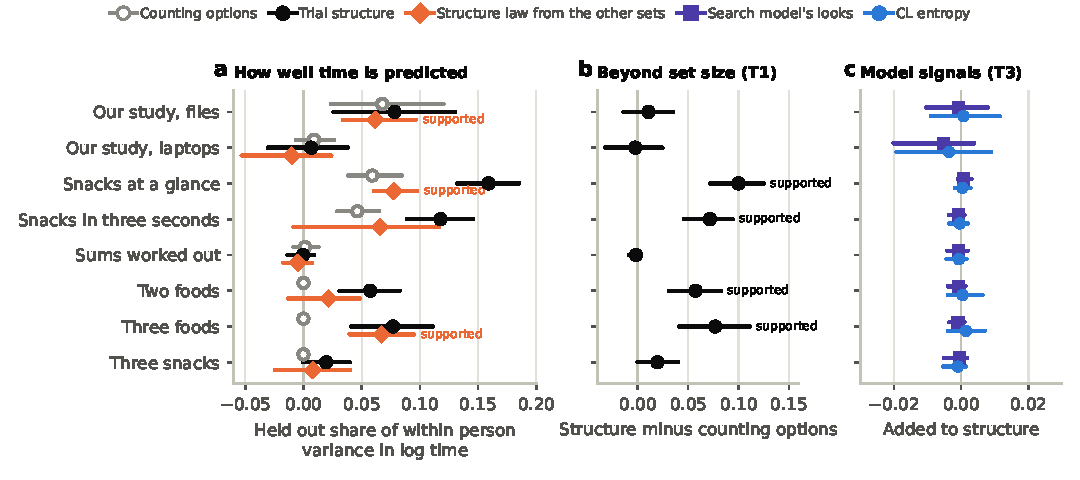
\includegraphics[width=\textwidth]{figures/figT1_structure.pdf}
\caption{Which trials take longer, from the structure of the trial (Amendment 12). This is Figure 5 of the paper, where the set size law is labelled counting options and the structure law trial structure. (a) Held out share of within person variance in log time for the set size law, the structure law and the structure law fitted to the other seven datasets, with 95 percent participant bootstrap intervals. (b) T1, structure minus the set size law. (c) T3, the gain from adding sample until return's expected looks to structure, and the gain from adding the entropy of CL's choice probabilities.}
\label{fig:structure}
\end{figure}

\begin{table}[t]
\centering
\footnotesize
\setlength{\tabcolsep}{4pt}
\caption{Which trials take longer, from the structure of the trial (Amendment 12, confirmatory). Held out share of within person variance in log time, ten folds of participants within each dataset, with 95 percent participant bootstrap intervals ($B = 1000$, refitted in every replicate). T1 is the structure law minus the set size law, T2 the score of a structure law fitted to the other seven datasets, T3 the gain from adding sample until return's expected looks to structure. An asterisk marks a test supported after Holm's correction across the eight datasets. BF$_{01}$ is the Bayes factor for no gain in T3.}
\label{tab:a12}
\begin{tabular}{lccccc}
\toprule
Dataset & Structure law & \makecell{T1, beyond\\set size} & \makecell{T2,\\transferred} & \makecell{T3, search\\looks added} & BF$_{01}$, T3 \\
\midrule
Our study, files & \makecell{$+0.078$ \\ {\scriptsize $[+0.026, +0.130]$}} & \makecell{$+0.011$ \\ {\scriptsize $[-0.014, +0.035]$}} & \makecell{$+0.062$\textsuperscript{*} \\ {\scriptsize $[+0.034, +0.097]$}} & \makecell{$-0.001$ \\ {\scriptsize $[-0.010, +0.008]$}} & $15.3$ \\
Our study, laptops & \makecell{$+0.007$ \\ {\scriptsize $[-0.031, +0.038]$}} & \makecell{$-0.002$ \\ {\scriptsize $[-0.032, +0.025]$}} & \makecell{$-0.010$ \\ {\scriptsize $[-0.053, +0.024]$}} & \makecell{$-0.005$ \\ {\scriptsize $[-0.020, +0.004]$}} & $18.5$ \\
Snacks at a glance & \makecell{$+0.159$ \\ {\scriptsize $[+0.132, +0.185]$}} & \makecell{$+0.100$\textsuperscript{*} \\ {\scriptsize $[+0.072, +0.125]$}} & \makecell{$+0.078$\textsuperscript{*} \\ {\scriptsize $[+0.060, +0.098]$}} & \makecell{$+0.001$ \\ {\scriptsize $[-0.001, +0.003]$}} & $27.7$ \\
Snacks in three seconds & \makecell{$+0.118$ \\ {\scriptsize $[+0.089, +0.146]$}} & \makecell{$+0.072$\textsuperscript{*} \\ {\scriptsize $[+0.046, +0.094]$}} & \makecell{$+0.066$ \\ {\scriptsize $[-0.009, +0.116]$}} & \makecell{$-0.001$ \\ {\scriptsize $[-0.004, +0.001]$}} & $75.5$ \\
Sums worked out & \makecell{$-0.000$ \\ {\scriptsize $[-0.014, +0.009]$}} & \makecell{$-0.002$ \\ {\scriptsize $[-0.009, +0.003]$}} & \makecell{$-0.005$ \\ {\scriptsize $[-0.017, +0.007]$}} & \makecell{$-0.001$ \\ {\scriptsize $[-0.004, +0.002]$}} & $61.9$ \\
Two foods & \makecell{$+0.057$ \\ {\scriptsize $[+0.031, +0.083]$}} & \makecell{$+0.057$\textsuperscript{*} \\ {\scriptsize $[+0.031, +0.083]$}} & \makecell{$+0.022$ \\ {\scriptsize $[-0.013, +0.048]$}} & \makecell{$-0.001$ \\ {\scriptsize $[-0.004, +0.001]$}} & $76.0$ \\
Three foods & \makecell{$+0.077$ \\ {\scriptsize $[+0.041, +0.111]$}} & \makecell{$+0.077$\textsuperscript{*} \\ {\scriptsize $[+0.041, +0.111]$}} & \makecell{$+0.067$\textsuperscript{*} \\ {\scriptsize $[+0.040, +0.095]$}} & \makecell{$-0.001$ \\ {\scriptsize $[-0.004, +0.001]$}} & $88.7$ \\
Three snacks & \makecell{$+0.019$ \\ {\scriptsize $[-0.000, +0.040]$}} & \makecell{$+0.019$ \\ {\scriptsize $[-0.000, +0.040]$}} & \makecell{$+0.008$ \\ {\scriptsize $[-0.024, +0.040]$}} & \makecell{$-0.000$ \\ {\scriptsize $[-0.005, +0.002]$}} & $40.6$ \\
\bottomrule
\end{tabular}
\end{table}


\paragraph{Structure predicts which trials take longer.} The structure law beat the set size law in four datasets (Figure~\ref{fig:structure}, Table~\ref{tab:a12}). In snacks at a glance T1 was $+0.100$ $[+0.072, +0.125]$, in snacks in three seconds $+0.072$ $[+0.046, +0.094]$, in two foods $+0.057$ $[+0.031, +0.083]$ and in three foods $+0.077$ $[+0.041, +0.111]$. With two or three options the set size law scores zero, so T1 there is the structure law's own score. In three snacks the structure law reached $+0.019$, with an interval just touching zero and an inconclusive Bayes factor (BF$_{01} = 0.52$). In our file task it reached $+0.011$ beyond set size (BF$_{01} = 2.07$). There the best value was fixed by design, which removes the feature that carries most of T1 elsewhere. In the sums and the laptop task structure added nothing (BF$_{01} = 30.5$ and $4.42$).

\paragraph{A law from other datasets carries over.} Fitted to the seven other datasets and applied unchanged, the structure law predicted which trials took longer in our file task ($+0.062$ $[+0.034, +0.097]$), snacks at a glance ($+0.078$ $[+0.060, +0.098]$) and three foods ($+0.067$ $[+0.040, +0.095]$). In snacks in three seconds it reached $+0.066$, but its percentile interval reached below zero, so the test was not passed although the Bayes factor favoured an effect (BF$_{01} = 0.20$). In two foods and three snacks the evidence was inconclusive (BF$_{01} = 0.93$ and $2.55$), and in the sums and the laptop task it favoured no transfer (16.8 and 4.56).

\paragraph{The search model's looks add nothing to structure.} Sample until return's expected looks added nothing in any dataset. Every T3 estimate lay within 0.006 of zero, and the Bayes factors favoured no gain, from 15.3 to 88.7. The entropy of CL's choice probabilities added nothing either (every estimate within 0.004 of zero, Figure~\ref{fig:structure}c).

\begin{table}[t]
\centering
\footnotesize
\setlength{\tabcolsep}{4pt}
\caption{How much time each feature of the trial adds, from a linear mixed model of log seconds on the four structure features with a random intercept and a random slope of $\log_2 n$ per participant (REML). Percent change in time per doubling of the set, without and with the value features in the model, with 95 percent Wald intervals. Standardized coefficients of the best value and the gap to the runner up are in standard deviations of within person log time per standard deviation of the feature. Marginal and conditional $R^2$ follow \citet{nakagawa2013}. The conditional $R^2$ includes how fast each person is. Features that do not vary within a dataset are left out (set size in the two and three option datasets, the best value in our study, the mean of the rest with two options).}
\label{tab:lmm}
\begin{tabular}{lcccccc}
\toprule
Dataset & \makecell{Time per\\doubling, \%} & \makecell{Adjusted for\\values, \%} & \makecell{Best value,\\standardized} & \makecell{Gap,\\standardized} & \makecell{$R^2$\\marginal} & \makecell{$R^2$\\conditional} \\
\midrule
Our study, files & \makecell{$23.1$ \\ {\scriptsize $[14.9, 32.0]$}} & \makecell{$44.5$ \\ {\scriptsize $[26.7, 64.9]$}} & -- & $+0.26$ & $0.046$ & $0.430$ \\
Our study, laptops & \makecell{$7.7$ \\ {\scriptsize $[1.0, 14.8]$}} & \makecell{$16.3$ \\ {\scriptsize $[6.1, 27.5]$}} & -- & $+0.13$ & $0.009$ & $0.504$ \\
Snacks at a glance & \makecell{$21.3$ \\ {\scriptsize $[17.5, 25.3]$}} & \makecell{$38.5$ \\ {\scriptsize $[33.7, 43.5]$}} & $-0.35$ & $+0.11$ & $0.150$ & $0.444$ \\
Snacks in three seconds & \makecell{$6.9$ \\ {\scriptsize $[5.6, 8.2]$}} & \makecell{$12.0$ \\ {\scriptsize $[10.3, 13.8]$}} & $-0.30$ & $+0.05$ & $0.110$ & $0.523$ \\
Sums worked out & \makecell{$17.0$ \\ {\scriptsize $[6.8, 28.1]$}} & \makecell{$20.1$ \\ {\scriptsize $[6.5, 35.5]$}} & $-0.01$ & $-0.00$ & $0.013$ & $0.282$ \\
Two foods & -- & -- & $-0.12$ & $-0.17$ & $0.050$ & $0.384$ \\
Three foods & -- & -- & $-0.28$ & $-0.03$ & $0.052$ & $0.557$ \\
Three snacks & -- & -- & $-0.21$ & $-0.01$ & $0.026$ & $0.289$ \\
\bottomrule
\end{tabular}
\end{table}


\paragraph{How large the effects are.} A linear mixed model with a random intercept and a random slope of set size for each participant gives the size of these effects (Table~\ref{tab:lmm}). Time grew by 21 percent for each doubling of the set in snacks at a glance, 7 percent in snacks in three seconds, 17 percent in the sums, 23 percent in our file task and 8 percent in our laptop task, all with intervals above zero. With the value features held fixed the growth was larger, 39 percent per doubling in snacks at a glance and 12 percent in three seconds. Larger trials held better best options (the mean best value rose from 0.92 of the scale with 9 snacks to 0.99 with 36, and from 0.81 to 0.92 in three seconds), and a better best option speeds the choice, so part of the cost of more options is hidden when values are ignored. After set size, the best value had the largest standardized effect in snacks at a glance ($-0.35$), snacks in three seconds ($-0.30$), three foods ($-0.28$) and three snacks ($-0.21$). In two foods the gap between the two options mattered more ($-0.17$), and in the sums no value feature mattered (every standardized effect within 0.03 of zero). The fixed effects explained 15 and 11 percent of the variance in snacks at a glance and snacks in three seconds and between 1 and 5 percent in the others (marginal $\Rtwo$, \citealp{nakagawa2013}).

\section{Predicting each trial's time with choice models (exploratory)}
\label{sec:models}

The structure law describes time but does not explain it. This part asks whether a model of the choice process, fitted mainly to choices, predicts the same regularities.

\subsection{A sealed vault and rounds of development}

Asking models to fit time, and changing them until they do, invites fitting noise. The work was therefore split before any fit. In every dataset a random 30 percent of the participants, drawn with a fixed seed, formed a vault. No vault trial was used to fit, select or tune anything. Models were developed on the remaining participants over three rounds. Each round was scored over ten folds of those participants and logged, with what changed and why, before the next round began. After the third round every model of the three rounds was frozen, 24 fitted models and calibrated versions of the 8 races, and the vault was opened once for all 32. The vault run was repeated and gave identical predictions, and separate code recomputed every vault $\Rtwo$ and the bootstrap intervals of the main comparisons (largest difference $10^{-15}$).

A rule for a satisfactory fit was fixed before any fit. A model is satisfactory when, on the vault, its score is clearly above the set size law in every dataset where the structure law is, and it is not clearly below the structure law in any dataset. Clear uses the same two intervals as above, from a bootstrap of vault participants without refitting ($B = 1000$). Comparisons with the structure law are also tested with a linear mixed model of the per trial difference in squared error, with a random intercept for each participant and Holm's correction across the eight datasets, and summarized by Cohen's $d_z$ of the per participant mean difference and by the share of vault participants whose predictions improved. Where a model is not clearly above structure, a Bayes factor weighs no gain against a half normal gain scaled to the development gain of structure over set size in that dataset (at least 0.01), and at half and double that scale.

\subsection{The models}
\label{sec:modellist}

\begin{table}[t]
\centering
\footnotesize
\setlength{\tabcolsep}{4pt}
\caption{The models compared on the vault. Choice parameters are fitted to the training participants' choices. Process races are fitted jointly to choices and to times divided by each person's geometric mean time. The round in which a model entered is given in brackets.}
\label{tab:models}
\begin{tabular}{p{2.6cm}p{6.2cm}p{6.6cm}}
\toprule
Group & Models & What predicts a trial's time \\
\midrule
Baselines & Set size law, structure law [1] & $\log_2 n$, or the four structure features, by least squares \\
Laws from choice models & CL, DbS and MLBA entropy, sample until return looks, two look satisficing looks [1], two look satisficing with its sensitivity chosen on time [2] & One quantity the choice model computes (entropy of its choice probabilities, or log expected looks) times one time slope \\
Process races & LBA, MLBA LBA, Wald race, relative Wald [1], each also with a threshold that rises with set size [2], each with and without one time slope [2] & The race's expected log time, from its joint fit to choices and times \\
Search timing & Sample until return timing [1] & Nondecision time plus a sum of gamma distributed look durations \\
Combined laws & Structure plus satisficing looks, plus sample until return looks, plus CL entropy [2], plus satisficing looks with sensitivity chosen on time, plus the Wald race with a rising threshold [3] & Structure features and one model quantity, by least squares \\
Ceilings & Boosted trees [1], boosted trees with centered features and inner tuning [2] & Thirteen trial features \\
\bottomrule
\end{tabular}
\end{table}

Table~\ref{tab:models} lists the models.

\paragraph{Time laws from choice models.} Each law takes a quantity $q$ that a choice model computes for the trial and predicts the centered time as $\beta q$, with the model's choice sensitivity fitted to the training choices and one time slope $\beta$ fitted by least squares. Entropy laws use the entropy in bits of the model's choice probabilities, as in Hick's law \citep{hick1952,hyman1953}, for CL, for decision by sampling scores \citep{stewart2006} and for averaged pairwise comparisons in the manner of MLBA. Looks laws use the log of a search model's expected number of looks.

\paragraph{Sample until return.} In sample until return (SR), each look falls on option $i$ with probability $q_i = e^{\lambda v_i} / \sum_j e^{\lambda v_j}$, and the search stops when some option receives its second look. That option is chosen. The expected number of looks is
\begin{equation}
\mathrm{E}[L_{\mathrm{SR}}] = \sum_{k=0}^{n} \Pr(L > k) = \sum_{k=0}^{n} k!\, e_k(q_1, \ldots, q_n),
\end{equation}
where $e_k$ is the elementary symmetric polynomial of degree $k$. A larger set takes more looks before the first repeat, so SR predicts that time grows with set size.

\paragraph{Two look satisficing.} Two look satisficing (TLS) adds an absolute standard to the same search \citep[in the spirit of][]{simon1955}. Looks fall on option $i$ with probability $\pi_i \propto e^{\lambda v_i / 2}$, and a look registers only with probability $h_i = e^{\lambda (v_i - 1)/2}$, which equals one for an option at the top of the value scale and is smaller the further an option lies below the top. The first option with two registered looks is chosen. Registered looks fall on option $i$ with probability $\pi_i h_i / \sum_j \pi_j h_j = q_i$, so TLS makes exactly the same choices as SR at the same $\lambda$. It takes
\begin{equation}
\mathrm{E}[L_{\mathrm{TLS}}] = \frac{\mathrm{E}[L_{\mathrm{SR}}]}{P}, \qquad P = \sum_i \pi_i h_i ,
\end{equation}
looks, where $P$ is the probability that a look registers. SR's looks do not change when every value in a trial moves by the same amount, because only differences in value enter $q$. TLS's looks do change. A trial whose options all lie far below the top of the scale registers few looks and takes longer. Both models have one choice sensitivity $\lambda$, fitted by maximum likelihood to the training choices, and one time slope. A variant chooses $\lambda$ instead from a grid of 30 values between 0.5 and 200 by the training score of its time law.

\paragraph{Process races.} Each race is fitted jointly to choices and times by maximum likelihood, the density of the chosen accumulator finishing first at the observed time, with each person's times divided by that person's geometric mean time so that speed does not enter the fit. LBA has drifts $d_0 + d_1 v_i$ with unit standard deviation, start points uniform on $[0, A]$, threshold $b = A + k$ and a nondecision time \citep{brown2008}. MLBA LBA replaces the drift with averaged weighted comparisons, $d_0 + g \sum_{j} w_{ij}(v_i - v_j)/(n-1)$ with $w_{ij} = e^{-l |v_i - v_j|}$ \citep{trueblood2014}. The Wald race uses racing diffusions with drifts $d_0 + d_1 v_i$, unit noise and threshold $b$ \citep{tillman2020}. The relative Wald race uses the drift $\nu / (1 + e^{-\tau (v_i - \max_{j \neq i} v_j)})$, the drift of the gaze weighted linear accumulator without gaze \citep{thomas2019}. In snacks in three seconds the likelihood is conditioned on a response before the limit. A race's prediction is its expected log time, computed by numerical integration, and its calibrated version multiplies that by one slope fitted on the training participants. From round 2 each race also had a version whose threshold grows as $b\, n^{\gamma}$ with $\gamma \geq 0$, one more parameter. Race accounts of Hick's law slow down with more options in this way, by raising the threshold to hold accuracy \citep{usher2002}.

\paragraph{Other models.} SR timing treats time as a nondecision time plus the sum of $L$ look durations, each gamma distributed, with $L$ drawn from SR at the sensitivity fitted to choices. Combined laws add one model quantity to the four structure features, to ask whether a model adds anything to structure. The two ceilings are boosted trees (scikit learn's HistGradientBoostingRegressor, \citealp{pedregosa2011}) trained on centered log time with thirteen trial features, namely $\log_2 n$, the five largest values, the gap, the mean and spread of the rest, the number of options within 0.1 of the best, and CL entropy at three fixed sensitivities. The second ceiling adds a within person centered copy of each feature and chooses its complexity by inner folds. A model's share of the better ceiling's score bounds its completeness for time in the sense of \citet{fudenberg2022}.

\paragraph{Checks on simulated data.} Before its first real fit, each process model was fitted to choices and times simulated from known parameters on the real displays of one dataset, with a speed factor for each person. The rising threshold races were checked this way before round 2. The fitted models recovered the true trial by trial expected log time ($\Rtwo$ between 0.92 and 0.99) and matched the held out score of the true model (Table~\ref{tab:sim}).

\subsection{What the development rounds changed}

\paragraph{Round 1.} Every model of the plan was run. Two look satisficing's looks alone matched or beat the structure law in snacks at a glance ($+0.168$ against $+0.162$) and in snacks in three seconds ($+0.128$ against $+0.123$). The races scored near or below zero wherever set size varied, down to $-0.667$ for LBA in snacks in three seconds. Their predictions correlated negatively with time within person ($r$ from $-0.07$ to $-0.30$). A race of independent accumulators with a fixed threshold finishes sooner when more accumulators run, so it predicts faster choices from larger trials, the opposite of what people do. With two or three options, where set size is fixed, the races' predictions correlated positively with time ($r$ from $+0.10$ to $+0.25$), and MLBA LBA scored $+0.049$, $+0.057$ and $+0.040$.

\paragraph{Round 2.} Six changes followed from round 1. Every race received a version whose threshold rises with set size, every race in snacks in three seconds was conditioned on the time limit, every race received a calibrated version, structure was combined with each of three model quantities, TLS's sensitivity was also chosen on time, and the ceiling was given centered features and inner tuning. The rising threshold Wald and relative Wald races improved on their fixed threshold versions wherever set size varies, for example the Wald race from $-0.241$ to $+0.070$ at a glance and from $-0.552$ to $+0.122$ in three seconds, where it now matched structure ($+0.123$), although both stayed slightly below zero in the sums. The time limit alone did not repair a fixed threshold (Wald race $-0.200$). The rising threshold LBA and MLBA LBA fits often failed to converge in development, which was found only after the vault was opened (Section~\ref{sec:refit}). Structure plus satisficing looks gave the best score in snacks at a glance ($+0.175$), and TLS with its sensitivity chosen on time the best in three seconds ($+0.131$).

\paragraph{Round 3.} Two combined laws were added. Structure plus satisficing looks with the sensitivity chosen on time lifted our file task from $+0.090$ to $+0.116$, close to the ceiling ($+0.120$). Structure plus the Wald race added nothing anywhere. Table~\ref{tab:dev} gives every development score.

\subsection{The vault}

\begin{figure}[t]
\centering
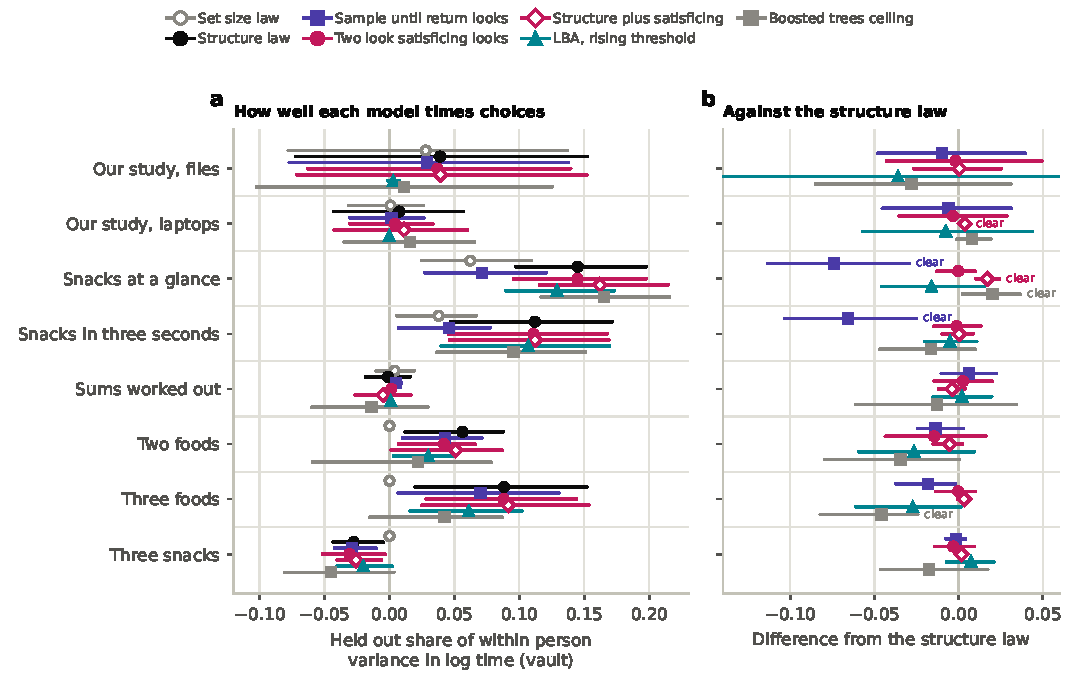
\includegraphics[width=\textwidth]{figures/figT3_vault.pdf}
\caption{Every main model scored once on the vault, after fitting on the other participants. (a) Held out share of within person variance in log time, with 95 percent bootstrap intervals over vault participants. (b) Each model's difference from the structure law. A label marks a difference whose percentile and basic intervals both exclude zero.}
\label{fig:vault}
\end{figure}

\begin{table}[t]
\centering
\footnotesize
\setlength{\tabcolsep}{2.6pt}
\caption{Held out $R^2$ of within person log time on the vault for the main models. Every model was fitted once on the participants outside the vault. Arrows mark a model clearly above or below the structure law (both 95 percent bootstrap intervals of the difference exclude zero). The structure law is clearly above the set size law in snacks at a glance, snacks in three seconds, two foods and three foods. Satisfactory follows the rule fixed before any fit. The rising threshold LBA race uses the corrected fit for snacks at a glance (Section~\ref{sec:refit}). Every model, with the frozen and the corrected fits, is in Table~\ref{tab:vaultall}.}
\label{tab:vaultmain}
\begin{tabular}{>{\raggedright\arraybackslash}p{3.4cm}ccccccccc}
\toprule
Model & \makecell{Our\\files} & \makecell{Our\\laptops} & \makecell{Snacks,\\glance} & \makecell{Snacks,\\3 s} & Sums & \makecell{Two\\foods} & \makecell{Three\\foods} & \makecell{Three\\snacks} & Satisfactory \\
\midrule
Set size law & $+0.028$ & $+0.001$ & $+0.062$\,$\downarrow$ & $+0.038$\,$\downarrow$ & $+0.004$ & $+0.000$\,$\downarrow$ & $+0.000$\,$\downarrow$ & $+0.000$\,$\uparrow$ & no \\
Structure law & $+0.039$ & $+0.008$ & $+0.145$ & $+0.112$ & $-0.001$ & $+0.056$ & $+0.088$ & $-0.028$ & yes \\
CL entropy & $+0.028$ & $+0.002$ & $+0.055$\,$\downarrow$ & $+0.044$\,$\downarrow$ & $+0.000$ & $+0.042$ & $+0.062$\,$\downarrow$ & $-0.033$\,$\downarrow$ & no \\
Sample until return looks & $+0.029$ & $+0.001$ & $+0.071$\,$\downarrow$ & $+0.046$\,$\downarrow$ & $+0.005$ & $+0.043$ & $+0.070$ & $-0.029$ & no \\
Two look satisficing looks & $+0.037$ & $+0.004$ & $+0.145$ & $+0.111$ & $+0.001$ & $+0.042$ & $+0.088$ & $-0.031$ & yes \\
Two look satisficing, sensitivity fitted to time & $+0.044$ & $+0.007$ & $+0.155$ & $+0.111$ & $+0.006$ & $+0.047$ & $+0.088$ & $-0.033$ & yes \\
Structure plus satisficing looks & $+0.039$ & $+0.011$\,$\uparrow$ & $+0.162$\,$\uparrow$ & $+0.112$ & $-0.005$ & $+0.051$ & $+0.091$ & $-0.026$ & yes \\
Structure plus sample until return looks & $+0.041$ & $-0.002$ & $+0.145$ & $+0.111$ & $-0.003$ & $+0.055$ & $+0.088$ & $-0.029$ & yes \\
Structure plus Wald race, rising threshold & $+0.032$ & $+0.021$\,$\uparrow$ & $+0.146$ & $+0.108$ & $-0.008$ & $+0.055$ & $+0.088$ & $-0.017$ & yes \\
LBA & $-0.065$ & $-0.171$ & $-0.050$\,$\downarrow$ & $+0.022$\,$\downarrow$ & $-0.037$ & $+0.012$ & $+0.047$ & $-0.098$\,$\downarrow$ & no \\
LBA, rising threshold, time slope & $+0.003$ & $-0.000$ & $+0.152$ & $+0.107$ & $+0.001$ & $+0.030$ & $+0.061$ & $-0.020$ & yes \\
Wald race, rising threshold & $+0.037$ & $-0.005$ & $+0.076$\,$\downarrow$ & $+0.097$ & $-0.001$ & $+0.024$ & $+0.048$ & $-0.077$\,$\downarrow$ & no \\
Boosted trees ceiling, centered features & $+0.011$ & $+0.016$ & $+0.165$\,$\uparrow$ & $+0.095$ & $-0.014$ & $+0.022$ & $+0.042$\,$\downarrow$ & $-0.045$ & no \\
\bottomrule
\end{tabular}
\end{table}


\paragraph{Seven models meet the rule.} The structure law was clearly above the set size law in snacks at a glance, snacks in three seconds, two foods and three foods, so these four datasets carried the first part of the rule (Figure~\ref{fig:vault}, Table~\ref{tab:vaultmain}). Seven of the 32 models met it, the structure law itself, two look satisficing with its sensitivity fitted to choices, two look satisficing with its sensitivity chosen on time, structure plus satisficing looks, structure plus sample until return's looks, structure plus the rising threshold Wald race, and the calibrated LBA race with a rising threshold. The last met it in the frozen run with a fit that had never left its starting values at a glance, and it still meets it with the best fit a fuller search found (Section~\ref{sec:refit}). No entropy law, no fixed threshold race, neither form of sample until return on its own and neither ceiling met it. Structure plus CL entropy fell clearly below structure in our laptop task and in three snacks, and structure plus satisficing looks with the sensitivity chosen on time was not clearly above zero in two foods.

\begin{table}[t]
\centering
\footnotesize
\setlength{\tabcolsep}{4pt}
\caption{Each model against the structure law on the vault, in the four datasets where structure beats set size. Difference in held out $R^2$ with its 95 percent bootstrap interval. Holm $p$ is from a linear mixed model of the per trial difference in squared error with a random intercept per participant, corrected across the eight datasets. $d_z$ is Cohen's effect size of the per participant mean difference, and Better is the percentage of vault participants whose predictions improved. BF$_{01}$ is the Bayes factor for no gain over structure, at the prior scale of the development gain of structure over set size and, in brackets, at half and double that scale. It is not computed where a model is clearly above structure.}
\label{tab:contrasts}
\begin{tabular}{>{\raggedright\arraybackslash}p{3.0cm}lcccccc}
\toprule
Model & Dataset & Difference & 95\% interval & Holm $p$ & $d_z$ & \makecell{Better,\\\%} & \makecell{BF$_{01}$\\$[\tfrac12, 2]$} \\
\midrule
Two look satisficing looks & Snacks, glance & $-0.000$ & $[-0.013, +0.010]$ & $1.00$ & $-0.05$ & $40$ & $18.7$ $[9.4, 37.3]$ \\
 & Snacks, 3 s & $-0.001$ & $[-0.015, +0.013]$ & $1.00$ & $-0.04$ & $38$ & $11.3$ $[5.7, 22.6]$ \\
 & Two foods & $-0.014$ & $[-0.044, +0.016]$ & $1.00$ & $-0.26$ & $42$ & $6.79$ $[3.6, 13.4]$ \\
 & Three foods & $-0.000$ & $[-0.014, +0.010]$ & $1.00$ & $-0.01$ & $44$ & $12.2$ $[6.2, 24.4]$ \\
\addlinespace
Structure plus satisficing looks & Snacks, glance & $+0.017$ & $[+0.010, +0.024]$ & $<0.001$ & $+1.15$ & $80$ & -- \\
 & Snacks, 3 s & $+0.000$ & $[-0.010, +0.009]$ & $1.00$ & $+0.02$ & $62$ & $14.4$ $[7.3, 28.8]$ \\
 & Two foods & $-0.005$ & $[-0.015, +0.002]$ & $1.00$ & $-0.37$ & $50$ & $28.2$ $[14.1, 56.3]$ \\
 & Three foods & $+0.003$ & $[-0.001, +0.006]$ & $0.66$ & $+0.53$ & $67$ & $2.88$ $[1.4, 5.8]$ \\
\addlinespace
Sample until return looks & Snacks, glance & $-0.074$ & $[-0.113, -0.030]$ & $0.02$ & $-0.78$ & $20$ & $23.2$ $[11.7, 46.3]$ \\
 & Snacks, 3 s & $-0.066$ & $[-0.103, -0.025]$ & $0.01$ & $-0.88$ & $8$ & $15.2$ $[7.7, 30.2]$ \\
 & Two foods & $-0.014$ & $[-0.024, +0.003]$ & $1.00$ & $-0.50$ & $25$ & $24.4$ $[12.3, 48.7]$ \\
 & Three foods & $-0.018$ & $[-0.037, -0.002]$ & $1.00$ & $-0.66$ & $22$ & $23.7$ $[11.9, 47.3]$ \\
\addlinespace
LBA, rising threshold, time slope & Snacks, glance & $-0.016$ & $[-0.045, +0.015]$ & $1.00$ & $-0.22$ & $53$ & $13.3$ $[6.8, 26.6]$ \\
 & Snacks, 3 s & $-0.005$ & $[-0.020, +0.011]$ & $1.00$ & $-0.15$ & $46$ & $14.1$ $[7.1, 28.1]$ \\
 & Two foods & $-0.027$ & $[-0.059, +0.009]$ & $1.00$ & $-0.39$ & $33$ & $7.70$ $[4.0, 15.2]$ \\
 & Three foods & $-0.027$ & $[-0.061, +0.002]$ & $0.70$ & $-0.57$ & $33$ & $12.2$ $[6.2, 24.3]$ \\
\addlinespace
Boosted trees ceiling, centered features & Snacks, glance & $+0.020$ & $[+0.002, +0.037]$ & $0.22$ & $+0.55$ & $67$ & -- \\
 & Snacks, 3 s & $-0.017$ & $[-0.047, +0.010]$ & $1.00$ & $-0.32$ & $46$ & $10.4$ $[5.3, 20.6]$ \\
 & Two foods & $-0.035$ & $[-0.080, +0.000]$ & $0.48$ & $-0.52$ & $25$ & $7.87$ $[4.1, 15.5]$ \\
 & Three foods & $-0.046$ & $[-0.082, -0.024]$ & $1.00$ & $-1.22$ & $11$ & $20.3$ $[10.2, 40.5]$ \\
\bottomrule
\end{tabular}
\end{table}


\paragraph{One choice parameter times decisions as well as four features.} Two look satisficing, with its sensitivity fitted to choices and one time slope, scored as well as the four feature structure law (Table~\ref{tab:contrasts}). In snacks at a glance it reached $+0.145$ $[+0.095, +0.198]$ against $+0.145$ $[+0.097, +0.198]$ for structure, in snacks in three seconds $+0.111$ against $+0.112$, and in three foods $+0.088$ against $+0.088$. The Bayes factors favoured no difference (BF$_{01} = 18.7$, $11.3$ and $12.2$, and above 5 at half the prior scale). In two foods it scored lower ($+0.042$ against $+0.056$), but not clearly (difference $-0.014$ $[-0.044, +0.016]$, BF$_{01} = 6.79$). It reached 88 percent of the better ceiling in snacks at a glance and exceeded both ceilings in the other three datasets, where the trees overfit.

\begin{figure}[t]
\centering
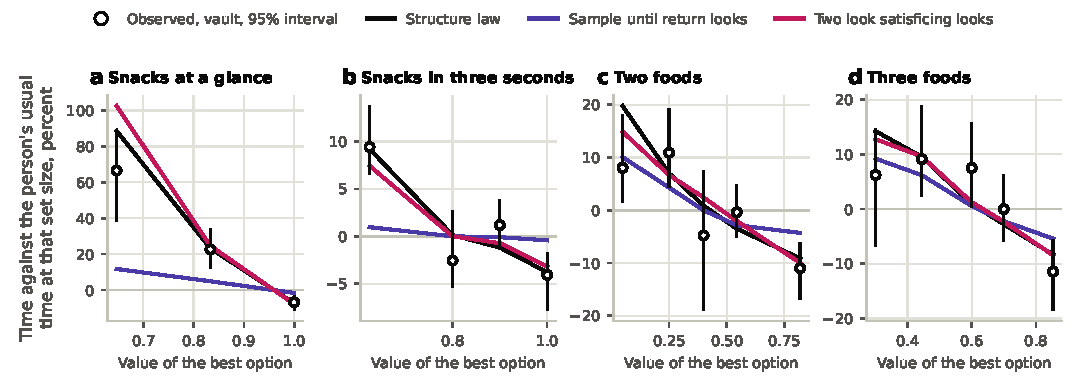
\includegraphics[width=\textwidth]{figures/figT5_bestvalue.pdf}
\caption{Time and the value of the best option on the vault, with the effect of set size removed. Each person's log time and each model's prediction are centered within person and then have their mean at each set size removed. Trials are binned in quintiles of the best option's value on the 0 to 1 scale. Ties at the top of the scale leave fewer than five bins in the snack datasets, and bins with fewer than 20 trials are not drawn. Points are observed means with 95 percent bootstrap intervals over vault participants.}
\label{fig:bestvalue}
\end{figure}

\paragraph{The absolute standard is what matters.} Sample until return makes exactly the same choices as two look satisficing at the same sensitivity, but its looks fell clearly below structure in snacks at a glance ($-0.074$ $[-0.113, -0.030]$) and in snacks in three seconds ($-0.066$ $[-0.103, -0.025]$). It already predicts the growth of time with set size (Figure~\ref{fig:setsize}). What it misses is the effect of values within a set size. Its looks depend on values only through their differences, so a trial of poor options takes as long as a trial of good ones, while people take longer when the best option is poor (Table~\ref{tab:lmm}). Figure~\ref{fig:bestvalue} shows this directly. With set size held fixed, people in snacks at a glance took 67 percent longer than usual on the trials with the lowest rated best snack and 7 percent less when the best snack was at the top of the scale. Sample until return's looks predicted $+12$ and $-2$ percent, two look satisficing $+103$ and $-8$, overshooting at the low end, and the structure law $+89$ and $-7$. In three seconds the pattern was the same (observed $+9$ and $-4$, sample until return $+1$ and $0$, two look satisficing $+7$ and $-3$). With two or three options sample until return's looks did fall as the best value rose, since a close pair takes more looks to separate, and both search models followed the data, two look satisficing more closely when the best option was good.

\paragraph{Satisficing adds to structure in the dataset it was built on.} Adding satisficing looks to structure improved on structure in snacks at a glance by $+0.017$ $[+0.010, +0.024]$ (Holm $p < 0.001$, $d_z = 1.15$, better for 80 percent of vault participants), reaching 98 percent of the better ceiling. Two look satisficing was first built on this dataset, so this gain is not a test on new data. In snacks in three seconds and two foods it equalled structure (BF$_{01} = 14.4$ and $28.2$). In three foods it gained $+0.003$, with a percentile interval reaching below zero and an inconclusive Bayes factor (2.88). In our laptop task it was clearly above structure, but by only $+0.004$ and with Holm $p = 0.43$ in the mixed model.

\paragraph{Races and ceilings.} With its best fit, the calibrated LBA race with a rising threshold scored $+0.152$ at a glance, level with structure ($+0.007$ $[-0.005, +0.022]$, BF$_{01} = 4.90$), and a little below structure in three seconds, two foods and three foods, never clearly (BF$_{01}$ from 7.69 to 14.1). It needs its time slope, which stretches the race's own predictions by a factor of 3.0 at a glance. The rising threshold Wald race fell clearly below structure at a glance ($+0.076$). Structure plus the Wald race added nothing in the four datasets where structure beats set size (BF$_{01}$ between 21.5 and 577) and was clearly above structure only in our laptop task ($+0.013$ $[+0.003, +0.023]$, Holm $p = 0.41$). The better ceiling was clearly above structure only in snacks at a glance ($+0.020$ $[+0.002, +0.037]$) and clearly below it in three foods ($-0.046$ $[-0.082, -0.024]$). No model and no ceiling explained more than 17 percent of the within person variance in any dataset.

\subsection{What a rising threshold does}

\begin{figure}[t]
\centering
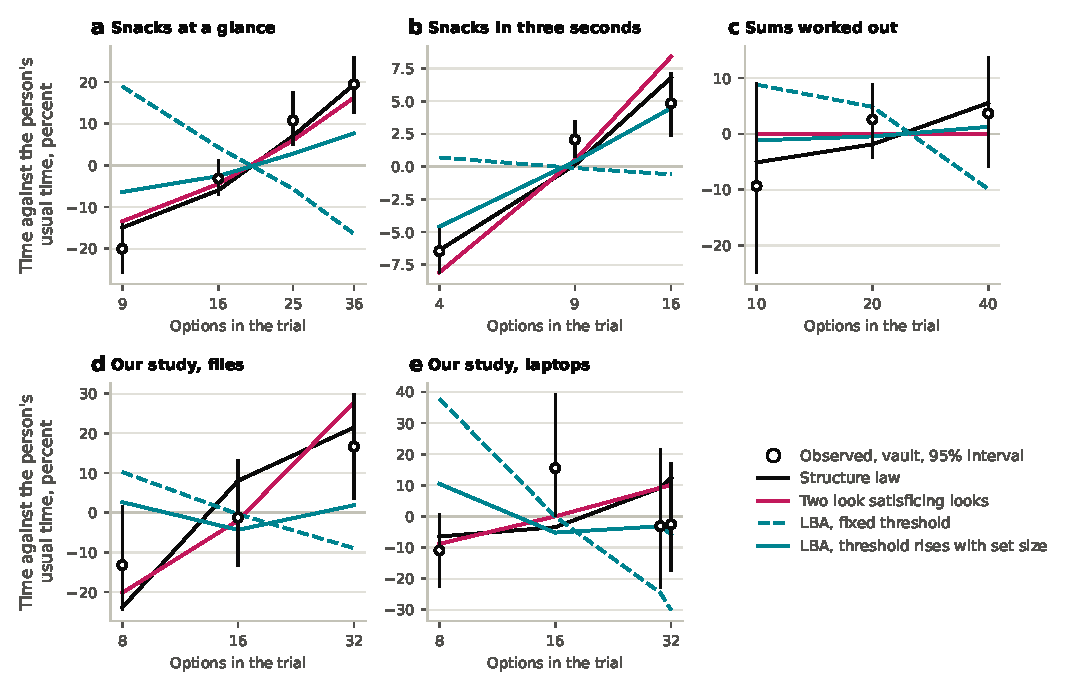
\includegraphics[width=\textwidth]{figures/figT2_setsize.pdf}
\caption{Mean decision time at each set size on the vault, against each person's usual time. Points are observed means with 95 percent bootstrap intervals over vault participants. Lines are the predictions of the structure law, two look satisficing's looks and the LBA race with a fixed threshold and with a threshold that rises with set size, both on the race's own time scale. The laptop task has sets of 30 and 32 options next to each other.}
\label{fig:setsize}
\end{figure}

Figure~\ref{fig:setsize} shows the problem. In snacks at a glance people took 20 percent less than their usual time with 9 snacks and 19 percent more with 36. The LBA race with a fixed threshold predicted the reverse, 19 percent more with 9 and 16 percent less with 36, and the fixed threshold Wald race predicted $+31$ and $-20$ percent. A threshold that grows as $b\,n^{\gamma}$ turned both around. For the Wald race the fitted exponent was $\gamma = 0.36$ at a glance and $0.24$ in three seconds. It needed no stretching by a time slope (slopes 0.99 and 1.16) and got the growth with set size right ($-18$ to $+23$ percent at a glance), but it captured less of the variation within a set size and scored about half of structure at a glance ($+0.076$). For LBA the exponent was $0.26$ at a glance and $0.42$ in three seconds. On its own time scale LBA still undershot the growth at a glance ($-6$ to $+7$ percent), and its time slope had to stretch its predictions by a factor of 3.0 to reach the observed range ($-18$ to $+22$ percent), against 1.6 in three seconds. In three seconds the fixed threshold LBA race conditioned on the limit predicted almost no change with set size, since the limit truncates its slow responses.

\subsection{Fitting problems found after the vault was opened}
\label{sec:refit}

\begin{table}[t]
\centering
\footnotesize
\setlength{\tabcolsep}{4pt}
\caption{Negative log likelihood of the vault fits of the two rising threshold races, on the training participants. Fixed is the nested fixed threshold race (ten starts for LBA, three for MLBA LBA), Frozen the fit of the frozen run and Final the fit used in this section. A rising threshold fit can never be worse than its fixed threshold version at a true optimum, so a frozen fit worse than the fixed one by more than 1 failed (dagger). For LBA, Final is the best admissible fit of the fuller search in every dataset, with its $\gamma$, which is not identified in the two and three option datasets because set size never changes there. For MLBA LBA, a frozen fit was replaced only where it failed, by a warm start refit that passed the check.}
\label{tab:convergence}
\begin{tabular}{lccccccc}
\toprule
 & \multicolumn{4}{c}{LBA, rising threshold} & \multicolumn{3}{c}{MLBA LBA, rising threshold} \\
\cmidrule(lr){2-5}\cmidrule(lr){6-8}
Dataset & Fixed & Frozen & Final & $\gamma$ & Fixed & Frozen & Final \\
\midrule
Our study, files & $1{,}448$ & $1{,}417$ & $1{,}417$ & $0.55$ & $1{,}450$ & $1{,}421$ & $1{,}421$ \\
Our study, laptops & $1{,}300$ & $1{,}263$ & $1{,}263$ & $0.60$ & $1{,}298$ & $1{,}264$ & $1{,}264$ \\
Snacks at a glance & $17{,}143$ & $164{,}548$\textsuperscript{\dag} & $16{,}986$ & $0.26$ & $17{,}290$ & $16{,}781$ & $16{,}781$ \\
Snacks in three seconds & $3{,}599$ & $3{,}540$ & $3{,}540$ & $0.42$ & $3{,}580$ & $3{,}432$ & $3{,}432$ \\
Sums worked out & $3{,}731$ & $3{,}721$ & $3{,}721$ & $1.11$ & $3{,}666$ & $42{,}060$\textsuperscript{\dag} & $3{,}665$ \\
Two foods & $3{,}188$ & $3{,}188$ & $3{,}188$ & $0.58$ & $2{,}824$ & $2{,}824$ & $2{,}824$ \\
Three foods & $2{,}769$ & $2{,}769$ & $2{,}769$ & $0.45$ & $2{,}527$ & $2{,}527$ & $2{,}527$ \\
Three snacks & $3{,}631$ & $3{,}631$ & $3{,}631$ & $0.45$ & $3{,}266$ & $3{,}266$ & $3{,}266$ \\
\bottomrule
\end{tabular}
\end{table}


The separate check of this section found that two vault fits had failed. A race whose threshold rises with set size contains its fixed threshold version as $\gamma$ approaches zero, so at a true optimum its likelihood can never be worse. The frozen fit of the rising threshold LBA race for snacks at a glance never left its starting values, with a negative log likelihood of 164{,}548 against 17{,}219 for the fixed threshold LBA, and the rising threshold MLBA LBA fit for the sums reached 42{,}060 against 3{,}666 (Table~\ref{tab:convergence}). Every other vault fit passed this check. In development the same two races failed in some folds, the rising LBA race in 8 of 10 folds in our file task, 5 in our laptop task, 8 in snacks at a glance and 1 in the sums, and the rising MLBA LBA race in 3 folds at a glance and 5 in the sums (Table~\ref{tab:dev}). The Wald races converged in every fold that could be checked. Snacks in three seconds could not be checked, because its round 2 fit records were overwritten when the fixed threshold races were rerun with the time limit.

Each step of the correction was logged before the vault was rescored with it, and every rule rests on likelihoods and stated bounds, not on vault scores. The scores of the first refit had been printed before its rule was refined, which the log records. The failed rising MLBA LBA fit in the sums was replaced by a refit started from the fixed threshold optimum, which moved its score from $-0.009$ to $+0.006$. For LBA the search had to go further, because the likelihood of the LBA family has several optima. A refit of every fixed threshold race with ten starts instead of three reached the frozen optimum everywhere except fixed LBA, which had stopped 75 short at a glance and 1.2 short in three seconds, and fixed MLBA LBA, 72 short at a glance. These fixed fits are kept as frozen and marked in Table~\ref{tab:vaultall}. At their fitted parameters all four fixed threshold races predict faster choices from larger trials in every dataset where set size varies, so a better optimum is unlikely to change their verdict. The rising threshold LBA race was refitted in every dataset from ten cold starts and from the ten start fixed optimum with $\gamma$ of 0.02, 0.3 and 0.7, keeping the best likelihood among fits whose expected log times are finite and within 50 of zero on the training and vault trials and whose $\gamma$ is at most 3. The bound excludes singular optima of the likelihood under the three second limit, which one start reached in three seconds ($\gamma = 15$, negative log likelihood $-57{,}334$), while every fit chosen in the other datasets had $\gamma$ of at most 1.1. At a glance the best fit has $\gamma = 0.26$ and a negative log likelihood of 16{,}986, against 17{,}059 for the best warm start from $\gamma = 0.02$ and 17{,}202 for ten cold starts. Every refit and search was run twice with identical results, and the corrected vault was evaluated twice and rechecked by separate code.

No verdict changes in the end. The calibrated rising threshold LBA race met the rule in the frozen run with an unfitted model ($+0.129$ at a glance) and meets it with its best fit ($+0.152$). An intermediate refit that stopped at a worse optimum ($\gamma = 0.01$, $+0.018$) would have reversed the verdict, so this race's result depends on which optimum its fit reaches and should be read with that in mind. The tables and figures of this section use the final fits, and Table~\ref{tab:vaultall} gives the frozen ones beside them. Two limits remain. The unseen set size measure of the rising LBA race uses refits that replace only fits failing the nesting check, without the fuller search, and the rising MLBA LBA race and the fixed LBA and MLBA LBA races were not searched further.

\subsection{Calibration}

\begin{figure}[t]
\centering
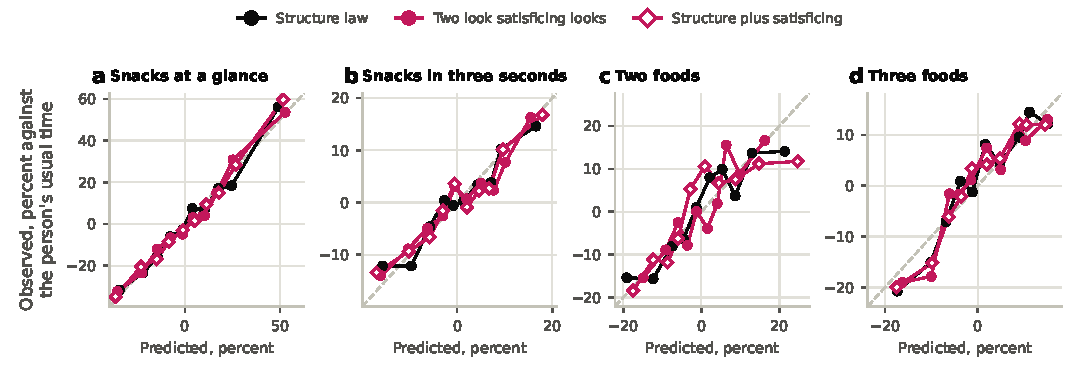
\includegraphics[width=\textwidth]{figures/figT4_calibration.pdf}
\caption{Calibration on the vault. Vault trials are binned in deciles of predicted time, and each point is the mean predicted and the mean observed time of a bin, as percent faster or slower than the person's usual time. Bins with fewer than 20 trials are not drawn. The dashed line is perfect calibration.}
\label{fig:calibration}
\end{figure}

The predictions were calibrated across the range of times (Figure~\ref{fig:calibration}). In snacks at a glance, the tenth of trials that two look satisficing predicted to take longest were predicted to take 53 percent longer than the person's usual time and took 54 percent longer, and the tenth predicted to be fastest were predicted at 36 percent and observed at 32 percent below the usual time. Regressing observed on predicted centered log time over all vault trials gave slopes near one, 1.00 for structure, 0.95 for two look satisficing and 0.99 for the two combined in snacks at a glance, 0.87, 0.86 and 0.82 in three seconds, 0.90, 1.00 and 0.83 in two foods, and 1.21, 1.26 and 1.25 in three foods.

\subsection{Secondary measures}

\begin{table}[t]
\centering
\footnotesize
\setlength{\tabcolsep}{3pt}
\caption{Secondary measures on the vault. (a) Mean within person rank correlation of predicted and observed time. (b) Bits per choice gained over a uniform guess on vault trials. Two look satisficing makes the same choices as sample until return.}
\label{tab:secondary}
\begin{tabular}{>{\raggedright\arraybackslash}p{4.4cm}cccccccc}
\toprule
\multicolumn{9}{l}{(a) Rank correlation with time} \\
\midrule
Model & \makecell{Our\\files} & \makecell{Our\\laptops} & \makecell{Snacks,\\glance} & \makecell{Snacks,\\3 s} & Sums & \makecell{Two\\foods} & \makecell{Three\\foods} & \makecell{Three\\snacks} \\
\midrule
Set size law & $+0.20$ & $+0.06$ & $+0.30$ & $+0.23$ & $+0.03$ & $+0.00$ & $+0.00$ & $+0.00$ \\
Structure law & $+0.23$ & $+0.11$ & $+0.39$ & $+0.36$ & $-0.05$ & $+0.22$ & $+0.28$ & $+0.07$ \\
Sample until return looks & $+0.23$ & $+0.07$ & $+0.30$ & $+0.25$ & $+0.09$ & $+0.19$ & $+0.25$ & $+0.07$ \\
Two look satisficing looks & $+0.23$ & $+0.10$ & $+0.39$ & $+0.35$ & $+0.07$ & $+0.18$ & $+0.28$ & $+0.02$ \\
Structure plus satisficing looks & $+0.22$ & $+0.11$ & $+0.41$ & $+0.36$ & $-0.04$ & $+0.22$ & $+0.28$ & $+0.06$ \\
LBA & $-0.15$ & $-0.02$ & $+0.05$ & $+0.18$ & $+0.06$ & $+0.16$ & $+0.22$ & $-0.01$ \\
Wald race & $-0.18$ & $-0.02$ & $-0.24$ & $-0.09$ & $-0.04$ & $+0.16$ & $+0.23$ & $-0.01$ \\
LBA, rising threshold, time slope & $+0.18$ & $-0.00$ & $+0.39$ & $+0.34$ & $+0.07$ & $+0.16$ & $+0.23$ & $-0.01$ \\
Wald race, rising threshold & $+0.20$ & $+0.10$ & $+0.34$ & $+0.34$ & $+0.01$ & $+0.16$ & $+0.22$ & $-0.01$ \\
Boosted trees ceiling, centered features & $+0.20$ & $+0.11$ & $+0.42$ & $+0.33$ & $+0.06$ & $+0.20$ & $+0.20$ & $+0.11$ \\
\midrule
\multicolumn{9}{l}{(b) Choices, bits per choice above a uniform guess} \\
\midrule
CL & $0.272$ & $0.617$ & $1.967$ & $0.754$ & $2.010$ & $0.240$ & $0.609$ & $0.298$ \\
Sample until return and two look satisficing & $0.272$ & $0.631$ & $1.964$ & $0.744$ & $2.015$ & $0.240$ & $0.610$ & $0.297$ \\
LBA & $0.276$ & $0.634$ & $1.889$ & $0.721$ & $2.139$ & $0.130$ & $0.487$ & $0.194$ \\
LBA, rising threshold & $0.273$ & $0.646$ & $1.541$ & $0.699$ & $2.142$ & $0.130$ & $0.487$ & $0.194$ \\
MLBA LBA & $0.278$ & $0.624$ & $1.922$ & $0.726$ & $2.217$ & $0.231$ & $0.615$ & $0.325$ \\
MLBA LBA, rising threshold & $0.279$ & $0.634$ & $1.872$ & $0.725$ & $0.917$ & $0.231$ & $0.615$ & $0.325$ \\
Wald race & $0.000$ & $0.093$ & $0.409$ & $0.650$ & $0.585$ & $0.117$ & $0.497$ & $0.188$ \\
Wald race, rising threshold & $0.000$ & $0.149$ & $0.572$ & $0.676$ & $0.708$ & $0.117$ & $0.497$ & $0.188$ \\
Relative Wald & $0.058$ & $0.412$ & $1.488$ & $0.754$ & $1.430$ & $0.233$ & $0.586$ & $0.293$ \\
Relative Wald, rising threshold & $0.075$ & $0.484$ & $1.488$ & $0.759$ & $1.299$ & $0.233$ & $0.586$ & $0.293$ \\
\bottomrule
\end{tabular}
\end{table}

\begin{table}[t]
\centering
\footnotesize
\setlength{\tabcolsep}{4pt}
\caption{Forecasting the time cost of a set size the model never saw, on the vault, in datasets with three or more set sizes. Each set size is left out in turn and every model is refitted on the others. Skill is one minus the mean squared error of each vault participant's predicted difference between mean log time at the left out size and at the other sizes, relative to forecasting no difference, with a 95 percent bootstrap interval. Negative skill is worse than forecasting no difference. Race refits at each left out size use three starts. A dagger marks the rising threshold LBA race, whose refits only replace fits that fail the nesting check, without the fuller search of Section~\ref{sec:refit}. A double dagger marks the two LBA races in the sums. With set size 20 left out, the fixed LBA refit stopped far from its optimum (negative log likelihood 8{,}115 against 2{,}237 with ten starts), and the rising LBA refit (2{,}488) passed the nesting check only against that failed fixed fit.}
\label{tab:unseen}
\begin{tabular}{>{\raggedright\arraybackslash}p{4.4cm}ccccc}
\toprule
Model & \makecell{Our\\files} & \makecell{Our\\laptops} & \makecell{Snacks,\\glance} & \makecell{Snacks,\\3 s} & Sums \\
\midrule
Set size law & \makecell{$-0.05$ \\ {\scriptsize $[-0.19, +0.20]$}} & \makecell{$-0.00$ \\ {\scriptsize $[-0.07, +0.05]$}} & \makecell{$+0.62$ \\ {\scriptsize $[+0.47, +0.70]$}} & \makecell{$+0.48$ \\ {\scriptsize $[-0.03, +0.69]$}} & \makecell{$+0.04$ \\ {\scriptsize $[-0.19, +0.17]$}} \\
Structure law & \makecell{$-26.59$ \\ {\scriptsize $[-55.69, -13.95]$}} & \makecell{$-1.36$ \\ {\scriptsize $[-2.27, -0.83]$}} & \makecell{$+0.55$ \\ {\scriptsize $[+0.35, +0.70]$}} & \makecell{$+0.17$ \\ {\scriptsize $[-0.49, +0.45]$}} & \makecell{$+0.05$ \\ {\scriptsize $[-0.19, +0.19]$}} \\
Sample until return looks & \makecell{$-0.06$ \\ {\scriptsize $[-0.20, +0.19]$}} & \makecell{$-0.00$ \\ {\scriptsize $[-0.07, +0.05]$}} & \makecell{$+0.63$ \\ {\scriptsize $[+0.48, +0.73]$}} & \makecell{$+0.43$ \\ {\scriptsize $[-0.20, +0.68]$}} & \makecell{$+0.02$ \\ {\scriptsize $[-0.02, +0.04]$}} \\
Two look satisficing looks & \makecell{$-0.15$ \\ {\scriptsize $[-0.34, +0.10]$}} & \makecell{$-0.01$ \\ {\scriptsize $[-0.08, +0.05]$}} & \makecell{$+0.64$ \\ {\scriptsize $[+0.52, +0.74]$}} & \makecell{$+0.43$ \\ {\scriptsize $[-0.41, +0.76]$}} & \makecell{$+0.00$ \\ {\scriptsize $[-0.00, +0.01]$}} \\
Structure plus satisficing looks & \makecell{$-3.20$ \\ {\scriptsize $[-6.99, -1.39]$}} & \makecell{$-1.87$ \\ {\scriptsize $[-3.21, -1.18]$}} & \makecell{$+0.60$ \\ {\scriptsize $[+0.46, +0.72]$}} & \makecell{$+0.31$ \\ {\scriptsize $[-0.26, +0.56]$}} & \makecell{$+0.04$ \\ {\scriptsize $[-0.19, +0.17]$}} \\
LBA & \makecell{$-0.65$ \\ {\scriptsize $[-1.63, -0.15]$}} & \makecell{$-0.46$ \\ {\scriptsize $[-0.81, -0.24]$}} & \makecell{$-1.96$ \\ {\scriptsize $[-2.62, -1.51]$}} & \makecell{$-0.63$ \\ {\scriptsize $[-1.08, -0.40]$}} & \makecell{$-0.32$\textsuperscript{\ddag} \\ {\scriptsize $[-0.68, -0.04]$}} \\
Wald race & \makecell{$-0.53$ \\ {\scriptsize $[-1.33, -0.13]$}} & \makecell{$-0.30$ \\ {\scriptsize $[-0.55, -0.15]$}} & \makecell{$-2.34$ \\ {\scriptsize $[-3.13, -1.95]$}} & \makecell{$-3.55$ \\ {\scriptsize $[-6.06, -2.42]$}} & \makecell{$-0.67$ \\ {\scriptsize $[-1.30, -0.14]$}} \\
LBA, rising threshold, time slope\textsuperscript{\dag} & \makecell{$-1.19$ \\ {\scriptsize $[-2.30, -0.74]$}} & \makecell{$-0.02$ \\ {\scriptsize $[-0.04, -0.00]$}} & \makecell{$-0.78$ \\ {\scriptsize $[-1.01, -0.62]$}} & \makecell{$+0.47$ \\ {\scriptsize $[-0.07, +0.70]$}} & \makecell{$-0.01$\textsuperscript{\ddag} \\ {\scriptsize $[-0.02, +0.00]$}} \\
Wald race, rising threshold & \makecell{$-0.07$ \\ {\scriptsize $[-0.21, +0.18]$}} & \makecell{$-0.02$ \\ {\scriptsize $[-0.08, +0.04]$}} & \makecell{$+0.62$ \\ {\scriptsize $[+0.43, +0.72]$}} & \makecell{$-6.09$ \\ {\scriptsize $[-9.91, -4.40]$}} & \makecell{$+0.04$ \\ {\scriptsize $[-0.42, +0.31]$}} \\
Boosted trees ceiling, centered features & \makecell{$+0.00$ \\ {\scriptsize $[-0.15, +0.12]$}} & \makecell{$+0.01$ \\ {\scriptsize $[-0.04, +0.04]$}} & \makecell{$+0.50$ \\ {\scriptsize $[+0.29, +0.64]$}} & \makecell{$+0.30$ \\ {\scriptsize $[+0.09, +0.46]$}} & \makecell{$+0.05$ \\ {\scriptsize $[-0.08, +0.13]$}} \\
\bottomrule
\end{tabular}
\end{table}


The plan named three secondary measures, computed on the vault for every frozen model (Tables~\ref{tab:secondary} and~\ref{tab:unseen}).

\paragraph{Ranking a person's trials.} The within person rank correlation of predicted and observed time told the same story as $\Rtwo$. In snacks at a glance it was 0.39 for structure, 0.39 for two look satisficing and 0.41 for the two combined, against 0.30 for the set size law and 0.30 for sample until return. In three seconds the same models reached 0.36, 0.35 and 0.36, against 0.23 and 0.25. The fixed threshold LBA race reached only 0.05 at a glance.

\paragraph{An unseen set size.} Each set size was left out in turn, every model was refitted on the other sizes, and the test was how much longer or shorter each vault participant's choices were at the left out size than at the others. In snacks at a glance the search models forecast this at least as well as the laws, with a skill of 0.64 $[0.52, 0.74]$ for two look satisficing and 0.63 for sample until return, against 0.62 for the set size law and 0.55 for the structure law. The fixed threshold races forecast the wrong direction (skill $-1.96$ for LBA and $-2.34$ for the Wald race). In three seconds the intervals were wide (two look satisficing 0.43 $[-0.41, 0.76]$, set size law 0.48 $[-0.03, 0.69]$), and the rising threshold Wald race failed badly ($-6.09$), mostly because it got the smallest sets wrong when they were left out. In our two tasks the structure law could not extrapolate at all (skill $-26.6$ for files and $-1.36$ for laptops), because each left out display had feature values outside the range of the displays it was fitted on, while the search models stayed between $-0.15$ and $0.00$. In the sums no model forecast the unseen sizes.

\paragraph{What timing costs in choices.} Two look satisficing makes the same choices as sample until return, which predicted vault choices as well as CL in every dataset (within 0.015 bits per choice). The races, fitted jointly to choices and times, mostly predicted choices worse than CL. LBA lost 0.08 bits per choice at a glance, 0.03 in three seconds, 0.11 in two foods and 0.12 in three foods. The Wald race lost far more at a glance (1.56 bits) and in our two tasks (0.27 and 0.52), but about as much as LBA in two and three foods (0.12 and 0.11). The main exception was the sums, where LBA predicted choices better than CL by 0.13 bits $[0.10, 0.16]$ and MLBA LBA by 0.21 $[0.14, 0.28]$. Smaller gains appeared for LBA in our laptop task ($+0.017$) and for MLBA LBA in three snacks ($+0.027$). That is about the size of the gap between CL and the machine learning ceiling for choices in the sums (about 0.2 bits), the dataset where judging is costly and overload outgrew every forecast. It was not a planned comparison and deserves its own test.

\subsection{Where the vault shows nothing}

In the sums no model explained as much as 1 percent of the within person variance on the vault (the best scored $+0.006$), and in both tasks of our study and in three snacks no model reached a clearly positive score, the ceilings included (Figure~\ref{fig:vault}a). The reasons differ. In the sums, time grows with set size (17 percent per doubling, Table~\ref{tab:lmm}), but set size and values explain almost none of the variation between a person's trials, in the full sample of Amendment 12, in development and on the vault. Working out a sum takes time that the sum's value does not reveal. In our file task time was predictable in the full sample (set size law $+0.068$ and structure law $+0.078$ in Amendment 12, both clear), but the vault intervals were too wide to show it ($[-0.072, +0.152]$ for structure). In the laptop task every model scored near zero throughout, apart from the uncalibrated fixed threshold races (down to $-0.17$ on the vault) and sample until return timing ($-0.04$), which scored below zero. Three snacks scored above zero in development (structure $+0.036$), but on its vault, the smallest of the eight, every model scored below $+0.006$ and most below zero. We read this as sampling noise in a small vault rather than as a failure of the models, but it means that three snacks supports no model.

\section{What the time results mean}

\paragraph{One quantity carries what the structure says.} In snacks at a glance, snacks in three seconds and three foods, adding satisficing looks to the structure law shrinks the coefficients of set size and of the best value toward zero. In the fits used for the vault in snacks at a glance, the coefficient of the best value fell from $-2.76$ to $-0.17$ and that of $\log_2 n$ from $0.32$ to $0.08$. In snacks in three seconds they fell from $-0.67$ to $-0.03$ and from $0.11$ to $-0.02$. In three foods the best value's coefficient fell from $-0.68$ to $-0.24$. So in these datasets the expected looks of a search with an absolute standard carry most of what set size and the best value say about time. This does not hold in two foods, where the best value's coefficient grew from $-0.34$ to $-1.14$ as the looks entered with a negative coefficient, or in the sums, where nothing predicts time. Search takes longer when the trial has many options, because the first repeat comes later, and when nothing on it is close to the top of the scale, because fewer looks register.

\paragraph{Relation to the confirmatory tests of time.} Two earlier confirmatory tests also concerned TLS and time. On the three gaze datasets (Amendment 6), TLS's law for absolute time, $\log(t_0 + \tau L)$ on uncentered log seconds, was no better than a constant time (difference in error $-0.0002$ $[-0.0054, +0.0056]$) and slightly worse than SR's by its percentile interval ($+0.0045$ $[+0.0001, +0.0106]$), and its within person rank correlation with time ($+0.19$) did not exceed SR's ($+0.21$). In Amendment 12, SR's looks added nothing to structure (T3). The vault agrees with both. On the gaze datasets TLS and SR scored alike (two foods $+0.042$ and $+0.043$, three foods $+0.088$ and $+0.070$, three snacks $-0.031$ and $-0.029$), and SR's looks added nothing to structure (Table~\ref{tab:vaultmain}). The difference lies in the trials with many options, where an absolute standard separates a trial of poor snacks from a trial of good ones. The Amendment 6 test also scored absolute times, whose variation is mostly how fast each person is, while this analysis scores which of a person's trials take longer.

\paragraph{Limits.} The work is exploratory. The vault guards against fitting the development rounds to noise, but two look satisficing itself was built on snacks at a glance, so the evidence that it times decisions as well as structure comes from snacks in three seconds and three foods, where it matched structure (BF$_{01} = 11.3$ and $12.2$) and which played no part in building it. The vaults of the gaze datasets are small, so not being clearly below structure is weak evidence on its own, and the Bayes factors carry the claim of equality. The models predict which trials take longer for a person, not how fast that person is, and TLS needs a time slope in addition to its choice sensitivity. The race models are harder to fit than the laws. The likelihood of the LBA family has several optima, a first refit stopped at a worse one, and the verdict on the calibrated rising threshold LBA race depends on which optimum its fit reaches (Section~\ref{sec:refit}). Finally, the explained variance is modest. The best model and the ceiling both stay below a sixth of the within person variance on the vault (and at or below 0.175 in development), so most of the variation between a person's trials is not predictable from set size and values with these models.

\bibliographystyle{apalike}
\bibliography{refs}

\appendix
\section{Supplementary tables}

\begin{table}[h]
\centering
\footnotesize
\caption{Recovery of the process models on simulated data, before each model's first real fit (before round 1, and before round 2 for the rising threshold races). Choices and times were simulated from known parameters on the real displays of snacks in three seconds (rising threshold races on snacks at a glance), with a speed factor for each person. Half the simulated people were fitted and the other half predicted. Columns give the $\Rtwo$ of the fitted model's expected log time against the true expected log time, the held out score of the fitted and of the true model on the simulated times, and the agreement of the numerical expectation with a Monte Carlo average.}
\label{tab:sim}
\begin{tabular}{lcccc}
\toprule
Model & \makecell{Fitted against\\true} & \makecell{Held out,\\fitted} & \makecell{Held out,\\true} & \makecell{Numerical against\\Monte Carlo} \\
\midrule
LBA & $0.983$ & $0.292$ & $0.289$ & $0.986$ \\
MLBA LBA & $0.962$ & $0.197$ & $0.201$ & $0.977$ \\
Wald race & $0.982$ & $0.212$ & $0.207$ & $0.983$ \\
Relative Wald & $0.949$ & $0.086$ & $0.078$ & $0.954$ \\
Sample until return timing & $0.924$ & $0.097$ & $0.085$ & $0.927$ \\
LBA, rising threshold & $0.988$ & $0.411$ & $0.414$ & $0.993$ \\
Wald race, rising threshold & $0.991$ & $0.491$ & $0.491$ & $0.996$ \\
\bottomrule
\end{tabular}
\end{table}

\begin{table}[p]
\centering
\scriptsize
\setlength{\tabcolsep}{2.6pt}
\caption{Development scores, held out $R^2$ of within person log time over ten folds of the participants outside the vault. Round 2 reran the four fixed threshold races in snacks in three seconds conditioned on the three second limit. Each round was logged before the next was run.}
\label{tab:dev}
\begin{tabular}{c>{\raggedright\arraybackslash}p{4.6cm}cccccccc}
\toprule
Round & Model & \makecell{Our\\files} & \makecell{Our\\laptops} & \makecell{Snacks,\\glance} & \makecell{Snacks,\\3 s} & Sums & \makecell{Two\\foods} & \makecell{Three\\foods} & \makecell{Three\\snacks} \\
\midrule
1 & Set size law & $+0.083$ & $+0.011$ & $+0.057$ & $+0.050$ & $+0.000$ & $+0.000$ & $+0.000$ & $+0.000$ \\
1 & Structure law & $+0.090$ & $+0.016$ & $+0.162$ & $+0.123$ & $-0.003$ & $+0.056$ & $+0.072$ & $+0.036$ \\
1 & CL entropy & $+0.088$ & $+0.010$ & $+0.061$ & $+0.056$ & $-0.002$ & $+0.053$ & $+0.053$ & $+0.040$ \\
1 & DbS entropy & $+0.082$ & $+0.011$ & $+0.052$ & $+0.049$ & $-0.000$ & $+0.016$ & $+0.000$ & $+0.002$ \\
1 & MLBA entropy & $+0.079$ & $+0.011$ & $+0.035$ & $+0.041$ & $+0.000$ & $-0.001$ & $+0.050$ & $-0.004$ \\
1 & Sample until return looks & $+0.085$ & $+0.011$ & $+0.074$ & $+0.056$ & $-0.001$ & $+0.045$ & $+0.056$ & $+0.042$ \\
1 & Two look satisficing looks & $+0.085$ & $+0.015$ & $+0.168$ & $+0.128$ & $-0.002$ & $+0.033$ & $+0.071$ & $+0.018$ \\
1 & Sample until return timing & $+0.088$ & $-0.030$ & $+0.073$ & $+0.003$ & $-0.081$ & $+0.022$ & $+0.037$ & $+0.028$ \\
1 & LBA & $-0.087$ & $-0.378$ & $+0.010$ & $-0.667$ & $-0.084$ & $+0.003$ & $+0.033$ & $-0.018$ \\
1 & MLBA LBA & $-0.033$ & $-0.347$ & $-0.154$ & $-0.577$ & $-0.003$ & $+0.049$ & $+0.057$ & $+0.040$ \\
1 & Wald race & $-0.374$ & $-0.302$ & $-0.241$ & $-0.552$ & $-0.058$ & $+0.015$ & $+0.040$ & $-0.006$ \\
1 & Relative Wald & $-0.347$ & $-0.168$ & $-0.122$ & $-0.165$ & $-0.035$ & $+0.044$ & $+0.028$ & $+0.009$ \\
1 & Boosted trees ceiling & $+0.117$ & $+0.001$ & $+0.093$ & $-0.052$ & $-0.006$ & $+0.034$ & $-0.005$ & $-0.088$ \\
\addlinespace
2 & Two look satisficing, sensitivity fitted to time & $+0.091$ & $+0.014$ & $+0.172$ & $+0.131$ & $-0.002$ & $+0.042$ & $+0.072$ & $+0.021$ \\
2 & LBA, with the time limit &  &  &  & $+0.019$ &  &  &  &  \\
2 & LBA, time slope, with the time limit &  &  &  & $+0.030$ &  &  &  &  \\
2 & LBA, rising threshold & $+0.026$ & $+0.002$ & $+0.057$ & $+0.112$ & $-0.082$ & $+0.003$ & $+0.033$ & $-0.018$ \\
2 & LBA, rising threshold, time slope & $+0.050$ & $+0.021$ & $+0.096$ & $+0.124$ & $-0.002$ & $+0.020$ & $+0.057$ & $+0.004$ \\
2 & MLBA LBA, with the time limit &  &  &  & $-0.041$ &  &  &  &  \\
2 & MLBA LBA, time slope, with the time limit &  &  &  & $+0.004$ &  &  &  &  \\
2 & MLBA LBA, rising threshold & $+0.007$ & $-0.026$ & $-0.036$ & $+0.040$ & $-0.020$ & $+0.049$ & $+0.057$ & $+0.040$ \\
2 & MLBA LBA, rising threshold, time slope & $+0.017$ & $+0.006$ & $+0.012$ & $+0.039$ & $-0.000$ & $+0.056$ & $+0.058$ & $+0.038$ \\
2 & Wald race, with the time limit &  &  &  & $-0.200$ &  &  &  &  \\
2 & Wald race, time slope, with the time limit &  &  &  & $+0.000$ &  &  &  &  \\
2 & Wald race, rising threshold & $+0.075$ & $+0.013$ & $+0.070$ & $+0.122$ & $-0.005$ & $+0.015$ & $+0.040$ & $-0.006$ \\
2 & Wald race, rising threshold, time slope & $+0.075$ & $+0.013$ & $+0.070$ & $+0.121$ & $+0.001$ & $+0.020$ & $+0.057$ & $+0.004$ \\
2 & Relative Wald, with the time limit &  &  &  & $-0.093$ &  &  &  &  \\
2 & Relative Wald, time slope, with the time limit &  &  &  & $+0.009$ &  &  &  &  \\
2 & Relative Wald, rising threshold & $+0.078$ & $+0.010$ & $+0.033$ & $+0.029$ & $-0.005$ & $+0.044$ & $+0.028$ & $+0.009$ \\
2 & Relative Wald, rising threshold, time slope & $+0.078$ & $+0.010$ & $+0.040$ & $+0.035$ & $-0.000$ & $+0.058$ & $+0.029$ & $+0.003$ \\
2 & Structure plus satisficing looks & $+0.095$ & $+0.004$ & $+0.175$ & $+0.126$ & $-0.002$ & $+0.058$ & $+0.071$ & $+0.035$ \\
2 & Structure plus sample until return looks & $+0.092$ & $+0.001$ & $+0.163$ & $+0.121$ & $-0.003$ & $+0.054$ & $+0.071$ & $+0.036$ \\
2 & Structure plus CL entropy & $+0.093$ & $-0.000$ & $+0.162$ & $+0.122$ & $-0.005$ & $+0.057$ & $+0.072$ & $+0.035$ \\
2 & Boosted trees ceiling, centered features & $+0.120$ & $+0.009$ & $+0.154$ & $+0.091$ & $-0.002$ & $+0.003$ & $+0.028$ & $-0.020$ \\
\addlinespace
3 & Structure plus satisficing looks, sensitivity fitted to time & $+0.116$ & $+0.001$ & $+0.173$ & $+0.126$ & $-0.009$ & $+0.059$ & $+0.072$ & $+0.037$ \\
3 & Structure plus Wald race, rising threshold & $+0.091$ & $+0.012$ & $+0.162$ & $+0.121$ & $-0.003$ & $+0.055$ & $+0.071$ & $+0.038$ \\
\bottomrule
\end{tabular}
\end{table}

\begin{table}[p]
\centering
\scriptsize
\setlength{\tabcolsep}{2.6pt}
\caption{Every frozen model on the vault, held out $R^2$ of within person log time. Arrows as in Table~\ref{tab:vaultmain}. A dagger marks a frozen fit that failed to converge, and a section sign a frozen fixed threshold fit that stopped short of its ten start optimum (by 75 and 1.2 for LBA at a glance and in three seconds, and by 72 for MLBA LBA at a glance), Section~\ref{sec:refit}. The last four rows give the final fits, which at three decimals differ from the frozen ones only where a dagger stands. In snacks in three seconds every race is conditioned on a response before the three second limit.}
\label{tab:vaultall}
\begin{tabular}{>{\raggedright\arraybackslash}p{3.9cm}ccccccccc}
\toprule
Model & \makecell{Our\\files} & \makecell{Our\\laptops} & \makecell{Snacks,\\glance} & \makecell{Snacks,\\3 s} & Sums & \makecell{Two\\foods} & \makecell{Three\\foods} & \makecell{Three\\snacks} & Satisfactory \\
\midrule
Set size law & $+0.028$ & $+0.001$ & $+0.062$\,$\downarrow$ & $+0.038$\,$\downarrow$ & $+0.004$ & $+0.000$\,$\downarrow$ & $+0.000$\,$\downarrow$ & $+0.000$\,$\uparrow$ & no \\
Structure law & $+0.039$ & $+0.008$ & $+0.145$ & $+0.112$ & $-0.001$ & $+0.056$ & $+0.088$ & $-0.028$ & yes \\
CL entropy & $+0.028$ & $+0.002$ & $+0.055$\,$\downarrow$ & $+0.044$\,$\downarrow$ & $+0.000$ & $+0.042$ & $+0.062$\,$\downarrow$ & $-0.033$\,$\downarrow$ & no \\
DbS entropy & $+0.027$ & $+0.001$ & $+0.054$\,$\downarrow$ & $+0.038$\,$\downarrow$ & $+0.004$ & $+0.012$\,$\downarrow$ & $+0.000$\,$\downarrow$ & $+0.005$\,$\uparrow$ & no \\
MLBA entropy & $+0.027$ & $-0.001$ & $+0.039$\,$\downarrow$ & $+0.030$\,$\downarrow$ & $+0.003$ & $+0.001$\,$\downarrow$ & $+0.053$\,$\downarrow$ & $-0.000$\,$\uparrow$ & no \\
Sample until return looks & $+0.029$ & $+0.001$ & $+0.071$\,$\downarrow$ & $+0.046$\,$\downarrow$ & $+0.005$ & $+0.043$ & $+0.070$ & $-0.029$ & no \\
Two look satisficing looks & $+0.037$ & $+0.004$ & $+0.145$ & $+0.111$ & $+0.001$ & $+0.042$ & $+0.088$ & $-0.031$ & yes \\
Two look satisficing, sensitivity fitted to time & $+0.044$ & $+0.007$ & $+0.155$ & $+0.111$ & $+0.006$ & $+0.047$ & $+0.088$ & $-0.033$ & yes \\
Sample until return timing & $+0.027$ & $-0.043$ & $+0.070$\,$\downarrow$ & $-0.031$\,$\downarrow$ & $-0.027$ & $+0.021$ & $+0.041$\,$\downarrow$ & $+0.001$\,$\uparrow$ & no \\
LBA & $-0.065$ & $-0.171$ & $-0.050$\,$\downarrow$\textsuperscript{\S} & $+0.022$\,$\downarrow$\textsuperscript{\S} & $-0.037$ & $+0.012$ & $+0.047$ & $-0.098$\,$\downarrow$ & no \\
LBA, time slope & $+0.014$ & $-0.004$ & $+0.011$\,$\downarrow$\textsuperscript{\S} & $+0.038$\,$\downarrow$\textsuperscript{\S} & $-0.003$ & $+0.030$ & $+0.061$ & $-0.020$ & no \\
LBA, rising threshold & $+0.013$ & $-0.016$ & $+0.068$\,$\downarrow$\textsuperscript{\dag} & $+0.096$ & $-0.021$ & $+0.012$ & $+0.047$ & $-0.098$\,$\downarrow$ & no \\
LBA, rising threshold, time slope & $+0.003$ & $-0.000$ & $+0.129$\textsuperscript{\dag} & $+0.107$ & $+0.001$ & $+0.030$ & $+0.061$ & $-0.020$ & yes \\
MLBA LBA & $-0.026$ & $-0.157$ & $-0.066$\,$\downarrow$\textsuperscript{\S} & $-0.032$\,$\downarrow$ & $+0.005$ & $+0.040$ & $+0.064$\,$\downarrow$ & $-0.023$ & no \\
MLBA LBA, time slope & $+0.029$ & $-0.004$ & $-0.002$\,$\downarrow$\textsuperscript{\S} & $+0.001$\,$\downarrow$ & $-0.004$ & $+0.039$ & $+0.066$\,$\downarrow$ & $-0.038$\,$\downarrow$ & no \\
MLBA LBA, rising threshold & $+0.001$ & $-0.008$ & $-0.057$\,$\downarrow$ & $+0.055$\,$\downarrow$ & $-0.009$\textsuperscript{\dag} & $+0.040$ & $+0.064$\,$\downarrow$ & $-0.023$ & no \\
MLBA LBA, rising threshold, time slope & $-0.022$ & $-0.000$ & $-0.004$\,$\downarrow$ & $+0.054$\,$\downarrow$ & $+0.004$\textsuperscript{\dag} & $+0.039$ & $+0.066$\,$\downarrow$ & $-0.038$\,$\downarrow$ & no \\
Wald race & $-0.352$\,$\downarrow$ & $-0.156$ & $-0.232$\,$\downarrow$ & $-0.154$\,$\downarrow$ & $-0.062$ & $+0.024$ & $+0.048$ & $-0.077$\,$\downarrow$ & no \\
Wald race, time slope & $+0.025$ & $+0.003$ & $+0.052$\,$\downarrow$ & $+0.004$\,$\downarrow$ & $+0.004$ & $+0.029$ & $+0.059$ & $-0.020$ & no \\
Wald race, rising threshold & $+0.037$ & $-0.005$ & $+0.076$\,$\downarrow$ & $+0.097$ & $-0.001$ & $+0.024$ & $+0.048$ & $-0.077$\,$\downarrow$ & no \\
Wald race, rising threshold, time slope & $+0.032$ & $-0.006$ & $+0.076$\,$\downarrow$ & $+0.094$ & $+0.004$ & $+0.029$ & $+0.059$ & $-0.020$ & no \\
Relative Wald & $-0.324$\,$\downarrow$ & $-0.075$ & $-0.098$\,$\downarrow$ & $-0.079$\,$\downarrow$ & $-0.033$ & $+0.035$ & $+0.036$\,$\downarrow$ & $-0.003$ & no \\
Relative Wald, time slope & $+0.022$ & $-0.000$ & $+0.037$\,$\downarrow$ & $+0.009$\,$\downarrow$ & $+0.004$ & $+0.038$ & $+0.041$\,$\downarrow$ & $-0.009$ & no \\
Relative Wald, rising threshold & $+0.040$ & $-0.003$ & $+0.051$\,$\downarrow$ & $-0.004$\,$\downarrow$ & $+0.002$ & $+0.035$ & $+0.036$\,$\downarrow$ & $-0.003$ & no \\
Relative Wald, rising threshold, time slope & $+0.035$ & $+0.000$ & $+0.052$\,$\downarrow$ & $+0.018$\,$\downarrow$ & $+0.005$ & $+0.038$ & $+0.041$\,$\downarrow$ & $-0.009$ & no \\
Structure plus satisficing looks & $+0.039$ & $+0.011$\,$\uparrow$ & $+0.162$\,$\uparrow$ & $+0.112$ & $-0.005$ & $+0.051$ & $+0.091$ & $-0.026$ & yes \\
Structure plus sample until return looks & $+0.041$ & $-0.002$ & $+0.145$ & $+0.111$ & $-0.003$ & $+0.055$ & $+0.088$ & $-0.029$ & yes \\
Structure plus CL entropy & $+0.040$ & $+0.002$\,$\downarrow$ & $+0.147$\,$\uparrow$ & $+0.112$ & $-0.002$ & $+0.056$ & $+0.093$ & $-0.030$\,$\downarrow$ & no \\
Structure plus satisficing looks, sensitivity fitted to time & $+0.014$ & $+0.013$ & $+0.160$\,$\uparrow$ & $+0.112$ & $-0.012$ & $+0.049$ & $+0.093$ & $-0.032$ & no \\
Structure plus Wald race, rising threshold & $+0.032$ & $+0.021$\,$\uparrow$ & $+0.146$ & $+0.108$ & $-0.008$ & $+0.055$ & $+0.088$ & $-0.017$ & yes \\
Boosted trees ceiling & $+0.007$ & $+0.013$ & $+0.110$\,$\downarrow$ & $-0.088$\,$\downarrow$ & $-0.004$ & $+0.023$ & $+0.036$ & $-0.167$\,$\downarrow$ & no \\
Boosted trees ceiling, centered features & $+0.011$ & $+0.016$ & $+0.165$\,$\uparrow$ & $+0.095$ & $-0.014$ & $+0.022$ & $+0.042$\,$\downarrow$ & $-0.045$ & no \\
\midrule
\multicolumn{10}{l}{Corrected fits, refitted after the vault was opened} \\
\midrule
LBA, rising threshold, corrected & $+0.013$ & $-0.016$ & $+0.086$\,$\downarrow$ & $+0.096$ & $-0.021$ & $+0.012$ & $+0.047$ & $-0.098$\,$\downarrow$ & no \\
LBA, rising threshold, time slope, corrected & $+0.003$ & $-0.000$ & $+0.152$ & $+0.107$ & $+0.001$ & $+0.030$ & $+0.061$ & $-0.020$ & yes \\
MLBA LBA, rising threshold, corrected & $+0.001$ & $-0.008$ & $-0.057$\,$\downarrow$ & $+0.055$\,$\downarrow$ & $+0.006$ & $+0.040$ & $+0.064$\,$\downarrow$ & $-0.023$ & no \\
MLBA LBA, rising threshold, time slope, corrected & $-0.022$ & $-0.000$ & $-0.004$\,$\downarrow$ & $+0.054$\,$\downarrow$ & $-0.004$ & $+0.039$ & $+0.066$\,$\downarrow$ & $-0.038$\,$\downarrow$ & no \\
\bottomrule
\end{tabular}
\end{table}


\FloatBarrier
\section{Reproducibility}

The plan for the model comparison and the log of every round were committed before the runs they describe. The vault was drawn with seed 20261103, the development folds with seed 20261014, and the vault bootstrap with seeds $130500 + b$. The files are listed below, all in the project repository.

{\raggedright
\begin{itemize}\setlength{\itemsep}{0pt}
\item Plan and log, \texttt{docs/time\_models\_plan.md} and \texttt{docs/time\_models\_log.md}
\item Amendment 12, \texttt{ANALYSIS\_PLAN.md} and \texttt{src/overload/experiments/time\_structure.py}
\item Models, \texttt{src/overload/time\_models.py}
\item Development and vault runs, \texttt{scripts/time\_models\_run.py} and \texttt{scripts/time\_models\_vault.sh}
\item Vault statistics, \texttt{scripts/time\_models\_vault\_eval.py}
\item Separate check of the vault numbers, \texttt{verification/check\_time\_vault.py}
\item Secondary measures, \texttt{scripts/time\_models\_secondary.py}
\item Mixed models and Bayes factors for Amendment 12, \texttt{scripts/stats\_misc.py} and \texttt{scripts/stats\_bayes.py}
\item Figures and tables of this section, \texttt{scripts/fig\_time\_writeup.py}, \texttt{scripts/fig\_time\_bestvalue.py} and \texttt{scripts/time\_writeup\_tables.py}
\end{itemize}
}

\end{document}
